\section{Lecture 37 - 12/5/2022}

\subsection{Common Mistakes on Midterm}

You are allowed to resubmit for the midterm! Please either send an email with the resubmitted programs or send a regrade request on Gradescope. Midterm Resubmission to due this Friday by \textbf{midnight}.\\

There were two common mistakes a lot of people had on the midterm:
\begin{enumerate}
    \item \textbf{Hyperbolic Disks: } There were some confusions on finding the Euclidean center of the disk. The idea is to first solve the question in the case where the hyperbolic center is $a = 0$:
    \[\fbox{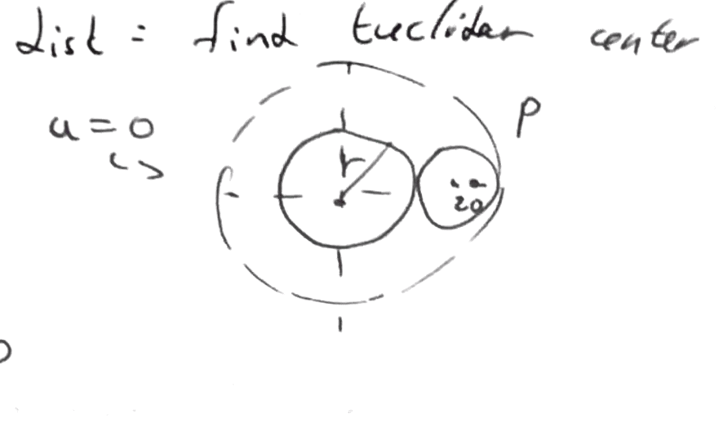
\includegraphics[width=.5\textwidth]{Figures/hyperbolic.png}}\]
    When $a = 0$, we have that
    \[\rho = \ln (\frac{1 + r}{1 - r})\]
    , and the Euclidean center coincide with the hyperbolic center. Now consider when $a = z_0$, then the following Mobius Transformation:
    \[z \mapsto \frac{z - z_0}{1 - \overline{z_0}z}\]
    maps hyperbolic disk to hyperbolic disk at the center. But note that $z_0$ is not the Euclidean center of its disks!\\\\
    It remains for us to find the Euclidean center of the disk, there are two ways to do this:
    \begin{itemize}
        \item Find $2$ points on the diameter opposite to each other
        \item Linear Fractional Transformation preserves symmetry, so Euclidean centers are symmetric to $\infty$, then we can find the inverse image of infinity, abd this map goes to $\frac{1}{\overline{z_0}}$
    \end{itemize}
    \item $f^N\ $ analytic \implies $f$ analytic: The common approach is first fix $z_0$ and write
    \[f(z)^N - f(z_0)^N = (f(z) - f(z_0)) \cdot (....)\]
    Then the claim is that if $f(z_0) \neq 0$, then $f(z)^N - f(z_0)^N$ be differentiable gives differentiability on $f(z) - f(z_0)$.\\\\
    In the case where $f(z_0) = 0$, we prove that the roots of $f$ are isolated and are in fact removable singularities.\\\\
    \textbf{There's another approach to this: }
    Let $U$ be some domain around $z_0$ small enough, then the $N$-th root of $z_0$ creates exactly $N$ regions whose $N$-th power goes to $U$:
    \[\fbox{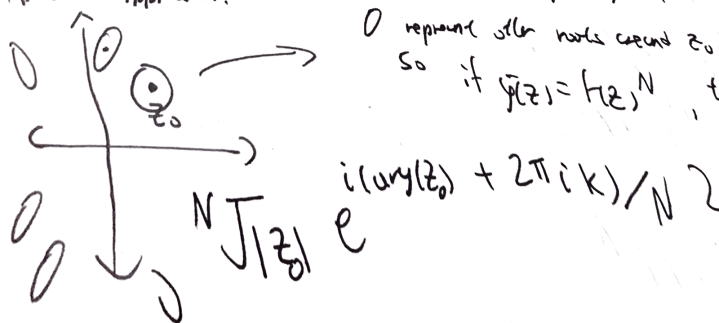
\includegraphics[width=.5\textwidth]{Figures/root.png}}\]
    In other words, if $g(z) = f(z)^N$, there exist analytic branches of $f(z) = g(z)^{1/N}$. We then claim that $f(z)$ must be in exactly ONE of these branches!\\\\
    This claim follows from the fact that each branch is connected, $f$ is continuous, and the continuous image of $f$ has to be connected.
\end{enumerate}

\subsection{Analytic Continuation}

Previously we have seen that functions like $\sqrt{1 - z^2}, \log(z)$ are not well-defined on the complex plane, as they are multi-valued functions. However, there's a way to make them well-defined by representing them on \textbf{Riemann surfaces} instead.\\

One notion to introduce Riemann Surfaces uses the idea of Analytic Continuation.\\

There's a naive approach to analytic continuation. Let $f \in Hol(\Omega)$ and consider some $z_0 \in \Omega$ as follows:
\[\fbox{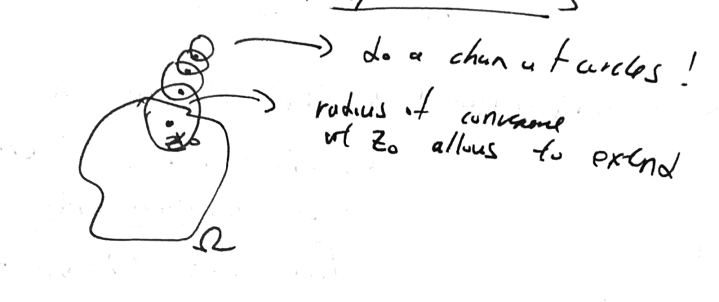
\includegraphics[width=.6\textwidth]{Figures/chain_circles.png}}\]
The idea is if the local power series at $z_0$ has radius of convergence greater than $d(z_0, \partial \Omega)$, then we could extend $f$ out of $\Omega$. If we can repeatedly do this, we can construct a chain of balls out of the boundary.\\

However, there are two problems with this approach:
\begin{enumerate}
    \item You are not always guaranteed that you can construct this chain of balls.
    \item Sometimes your extension may not match up with one another. For example take $f = \sqrt{z}$ with $\Omega$ being on the right half-plane:
    \[\fbox{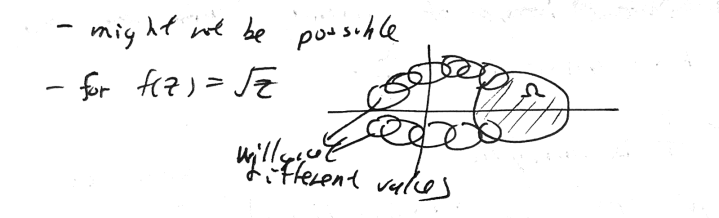
\includegraphics[width=.6\textwidth]{Figures/chain_root.png}}\]
    If you take a chain of circles going from the clock-wise and counter-clockwise direction, they WILL not give the same value when they meet.
\end{enumerate}

Therefore, we need a more standard way to discuss analytic continuation, and this leads to the idea of analytic continuation along a path.

\begin{definition}[Analytic Continuation Along a Path]
    Let $\gamma: [a, b] \to \Cbb$ be a path, we say that an \textbf{analytic continuation exists along $\gamma$} if there exist a family of $(f_s, U_s)$, $s \in [a, b]$ such that
    \[\gamma(s) \in U_s, f_s \in \text{Hol}(U_s)\]
    and for all $t_0 \in [a, b]$, there exist $\delta > 0$ such that
    \[|t - t_0| < \delta \implies \begin{cases}
    1.\ U_t \cap U_{t_0} \neq \emptyset\\
    2.\ f_t \equiv f_{t_0} \text{ on } U_t \cap U_{t_0}
    \end{cases}\]
\end{definition}

\begin{remark}
    In practice, once we have the family of functions, we will simplify $f_t$ as
    \[f_t(z) = \sum_0^\infty a_k(t) (z - \gamma(t))^k\]
    as a power series and take $U_t$ as a disk instead.
\end{remark}

\begin{proposition}
    Let $\gamma: [a, b] \to \Cbb$ be a path, an \textbf{analytic continuation exists along $\gamma$} if and only if there exists a finite division of $[a, b]$ into intervals $I_1, ..., I_n$ and family $(f_i, U_i)_{i = 1}^n$ such that
    \begin{itemize}
        \item $\gamma(I_k) \subseteq U_k$
        \item $U_k \cap U_{k+1} \neq \emptyset$
        \item $f_k \equiv f_{k+1}$ on $U_k \cap U_{k+1}$
    \end{itemize}
\end{proposition}

\begin{proof}
    Converse is straight-forward, for all $t \in [a, b]$, just choose $g_t$ to be $f_k$ if $t \in I_k$, then we have $(g_t, U_t)$ to be a valid family.\\\\
    For the forward, direction, consider $U_t$ for each $t \in [a, b]$ and
    \[\bigcup_{t \in [a, b]} \gamma^{-1}(U_t) \text{ is a cover of } [a, b]\]
    Then the Lebesgue Number's Lemma implies that there exists some $\alpha > 0$ such that for any $E \subseteq [a, b]$ where $diam(E) < \alpha$, there exist $U_t$ such that $E \subset \varphi^{-1}(U_t)$.\\\\
    Then we split intervals of $[a, b]$ to intervals $I_1, ..., I_n$ each less than $\alpha$ in length. Then for $I_k = [a_{k-1}, a_k]$ we have that $I_k \subseteq \gamma^{-1}(U_{t_k})$, hence $\gamma(I_k) \subseteq U_{t_k}$.\\\\
    Then the family $(f_{t_k}, U_{t_k})$ is our desired finite division.
\end{proof}

\begin{proposition}
    Analytic Continuation along a path is independent of the choice of splitting. In other words, the analytic continuation is unique.
\end{proposition}

\begin{proof}
    This follows from the Uniquenss Theorem of analytic functions. Suppose we have a finite splitting ${I_k}, {J_j}$ of $[a, b]$, then we can consider the splitting $\{I_k \cap I_j\}$ of $[a, b]$. This is a finer splitting than both given, then we apply the Uniqueness Theorem.
\end{proof}

\begin{definition}[Germs of Analytic Functions]
    Let $z_0 \in \Cbb$, then this consider the set of the form:
    \[S = \{(f, U)\ |\ \text{$f \in \text{Hol}(U)$, $U$ is a neighborhod of $z_0$}\}\]
    We can define an equivalence relation as follows, where $(f, U) \sim (g, V)$ if there exists some neighborhood $W \subseteq U \cap V$ containing $z_0$ such that $f \equiv g$ on $W$.\\\\
    This equivalence class is called the \textbf{germ of analytic functions at $z_0$}, which we denote an element of this class as $[f]_{z_0}$ and call it the \textbf{germ of $f$ at $z_0$}.
\end{definition}

\begin{remark}
    If $U, V$ are connected and convex domains, we can without loss take $W = U \cap V$. Analytic continuation being unique is essentially saying that our germs coincides along the path.
\end{remark}

\subsection{Monodromy's Theorem}
\begin{theorem}[Monodromy's Theorem]
    Suppose $\gamma_0, \gamma_1: [a, b] \to \Cbb$ are homotopy pathes with same start and end points, meaning there exist a continuous function $\Gamma(t, s): [a, b] \to [0, 1] \to \Cbb$ such that
    \[\Gamma(t, 0) = \gamma_0(t), \Gamma(t, 1) = \gamma_1(t), \Gamma(a, s) = z_0, \Gamma(b, s) = z_1\]
    Define $\gamma_s(t) \coloneqq \Gamma(t, s)$ for all $s \in [a, b]$. Suppose there exists analytic continuation along all of $\gamma_s(t)$ for some analytic function $f$, then the analytic continuation of $[f]_{\gamma_s(b)}$ is independent on $s$!
\end{theorem}

\begin{proof}[Idea]
    If two analytic continuations are ``close enough", they are the same.
\end{proof}

\begin{example}
    Take $f = \sqrt{z}$ on the principle branch, consider the two following ways to draw pathes from $\gamma_0(a) = 1$ to $\gamma_0(b) = -1$:
    \[\fbox{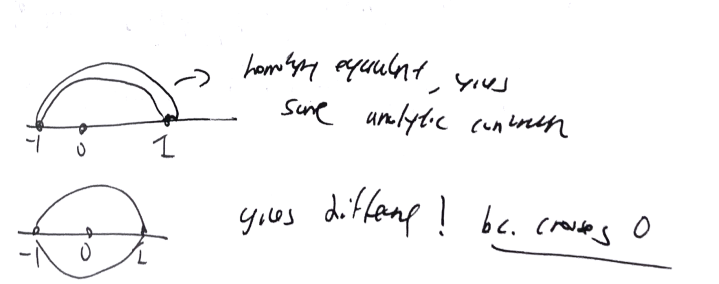
\includegraphics[width=.6\textwidth]{Figures/sqrt_root.png}}\]
    The pathes in the top figure are homotopy equivalent, the pathes in the bottom figure are not.
\end{example}